\begin{figure}[t]
\centering
\begin{tikzpicture}
\begin{axis}[
  width=0.82\linewidth, height=5.2cm,
  xlabel={sequence length $T$ (tokens)}, ylabel={state bytes per layer (MiB, bf16)},
  xmin=0, xmax=16384, ymin=0, ymax=50,
  xtick={0,4096,8192,12288,16384}, scaled x ticks=false,
  legend pos=north west, legend style={font=\footnotesize,draw=none,fill=none},
  tick label style={font=\footnotesize}, label style={font=\small}]
% KV cache: 2 T d_model b bytes, d_model=768, b=2  -> 3072 T bytes
\addplot[very thick,red!70!black,domain=0:16384,samples=2] {3072*x/1048576};
\addlegendentry{softmax KV-cache, $2Td_{\text{model}}b$ ($d_{\text{model}}{=}768$)}
% bounded state: n d b = 32768*256*2 bytes = 16 MiB
\addplot[very thick,blue!70!black,domain=0:16384,samples=2] {16};
\addlegendentry{BDH-GPU state, $ndb$ ($n{=}32{,}768$, $d{=}256$)}
\draw[dashed,gray] (axis cs:5461.33,0) -- (axis cs:5461.33,16);
\fill (axis cs:5461.33,16) circle (1.6pt);
\node[font=\footnotesize,anchor=north west] at (axis cs:5600,15.5) {$T^\star=\tfrac{nd}{2d_{\text{model}}}\approx5{,}461$};
\node[font=\scriptsize,gray,align=center] at (axis cs:2600,24) {bounded state\\is larger};
\node[font=\scriptsize,gray,align=center] at (axis cs:12200,8) {bounded state\\is smaller};
\end{axis}
\end{tikzpicture}
\caption{Byte crossover (\cref{eq:crossover}). KV-cache bytes grow linearly in $T$; the BDH-GPU state is constant at
$ndb=16$\,MiB per layer in bf16. Below $T^\star\approx5{,}461$ tokens the bounded state is the \emph{larger} memory.
Analytic, per layer and per sequence; it ignores activations, batching, and KV-cache compression.}
\label{fig:crossover}
\end{figure}
